\chapter{Umsetzung Beispiel}\label{chapter:Beispiel}

Dieses Kapitel präsentiert die praktische Umsetzung der in dieser Arbeit entwickelten Open Source Lakehouse Architektur. Dabei werden die zentralen Features, die verwendeten Skripte sowie die Integration und Funktionalität der einzelnen Komponenten näher erläutert.

Für die Analyse, Verarbeitung und Visualisierung dient der Datensatz \texttt{ds\_salaries.csv} als Grundlage. Dieser Datensatz umfasst insgesamt 11 Spalten, die detaillierte Informationen zu Gehältern, Arbeitsbedingungen und Unternehmensstrukturen enthalten. Er ist online unter folgender URL verfügbar: \url{https://www.kaggle.com/datasets/arnabchaki/data-science-salaries-2023} und in der bereitgestellten Abgabe im Ordner \texttt{spark/data} hinterlegt.

Die 11 Spalten des Datensatzes beinhalten die folgenden Informationen:
\begin{figure}[H]
    \centering
    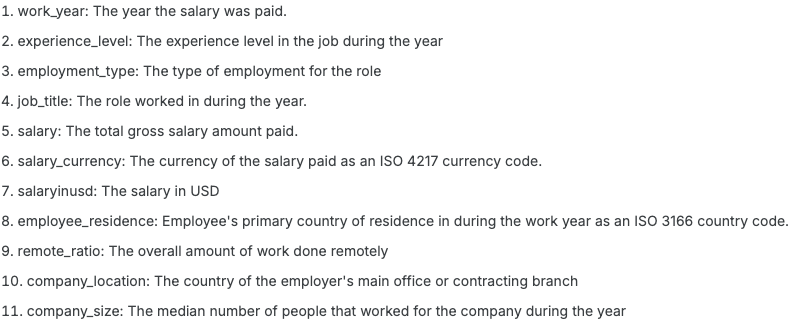
\includegraphics[width=1\linewidth]{graphics/datensatz.png}
    \caption[Beschreibung der Spalten des Datensatzes]{Beschreibung der Spalten des Datensatzes.}
    \label{fig:Datensatz-Kaggle}
\end{figure}

Um den Datensatz weiter anzureichern und die Möglichkeiten der Echtzeitverarbeitung zu demonstrieren, wurde zusätzlich ein Web-Scraper entwickelt. Dieser sammelt Gehaltsdaten von der Webseite Glassdoor unter folgender URL: \url{https://www.glassdoor.de/Job/Data-Scientist-jobs-SRCH_KO0,10.htm} und integriert die gesammelten Informationen direkt in den bestehenden Datensatz. Auf diese Weise werden die Analysen um zusätzliche Aspekte ergänzt, die eine Echtzeitverarbeitung sowie eine erweiterte Visualisierung der Daten ermöglichen. Der Web-Scraper befindet sich im Ordner \lstinline|scraper| und kann durch das Starten des entsprechenden Containers ausgeführt werden.

\newpage

\section{Demonstration von Features}

Die Umsetzung der Lakehouse-Architektur umfasst mehrere Schritte und Features. Zu Beginn wird ein \lstinline|minio|-Container gestartet, der als zentraler Objektspeicher dient. Anschließend erfolgt die Einrichtung durch einen \lstinline|minio-init|-Container. Während dieses Prozesses wird ein Administrator-Konto erstellt, dessen Zugangsdaten aus der \lstinline|.env|-Datei ausgelesen werden. Zudem wird ein Bucket mit dem Namen \lstinline|lakehouse-storage| konfiguriert, der als Speicherort für die verarbeiteten Daten dient.

Abbildung \ref{fig:MinIO-Login} zeigt den Login-Bildschirm von MinIO, der den Zugang zur Verwaltungsoberfläche ermöglicht. 

\begin{figure}[H]
    \centering
    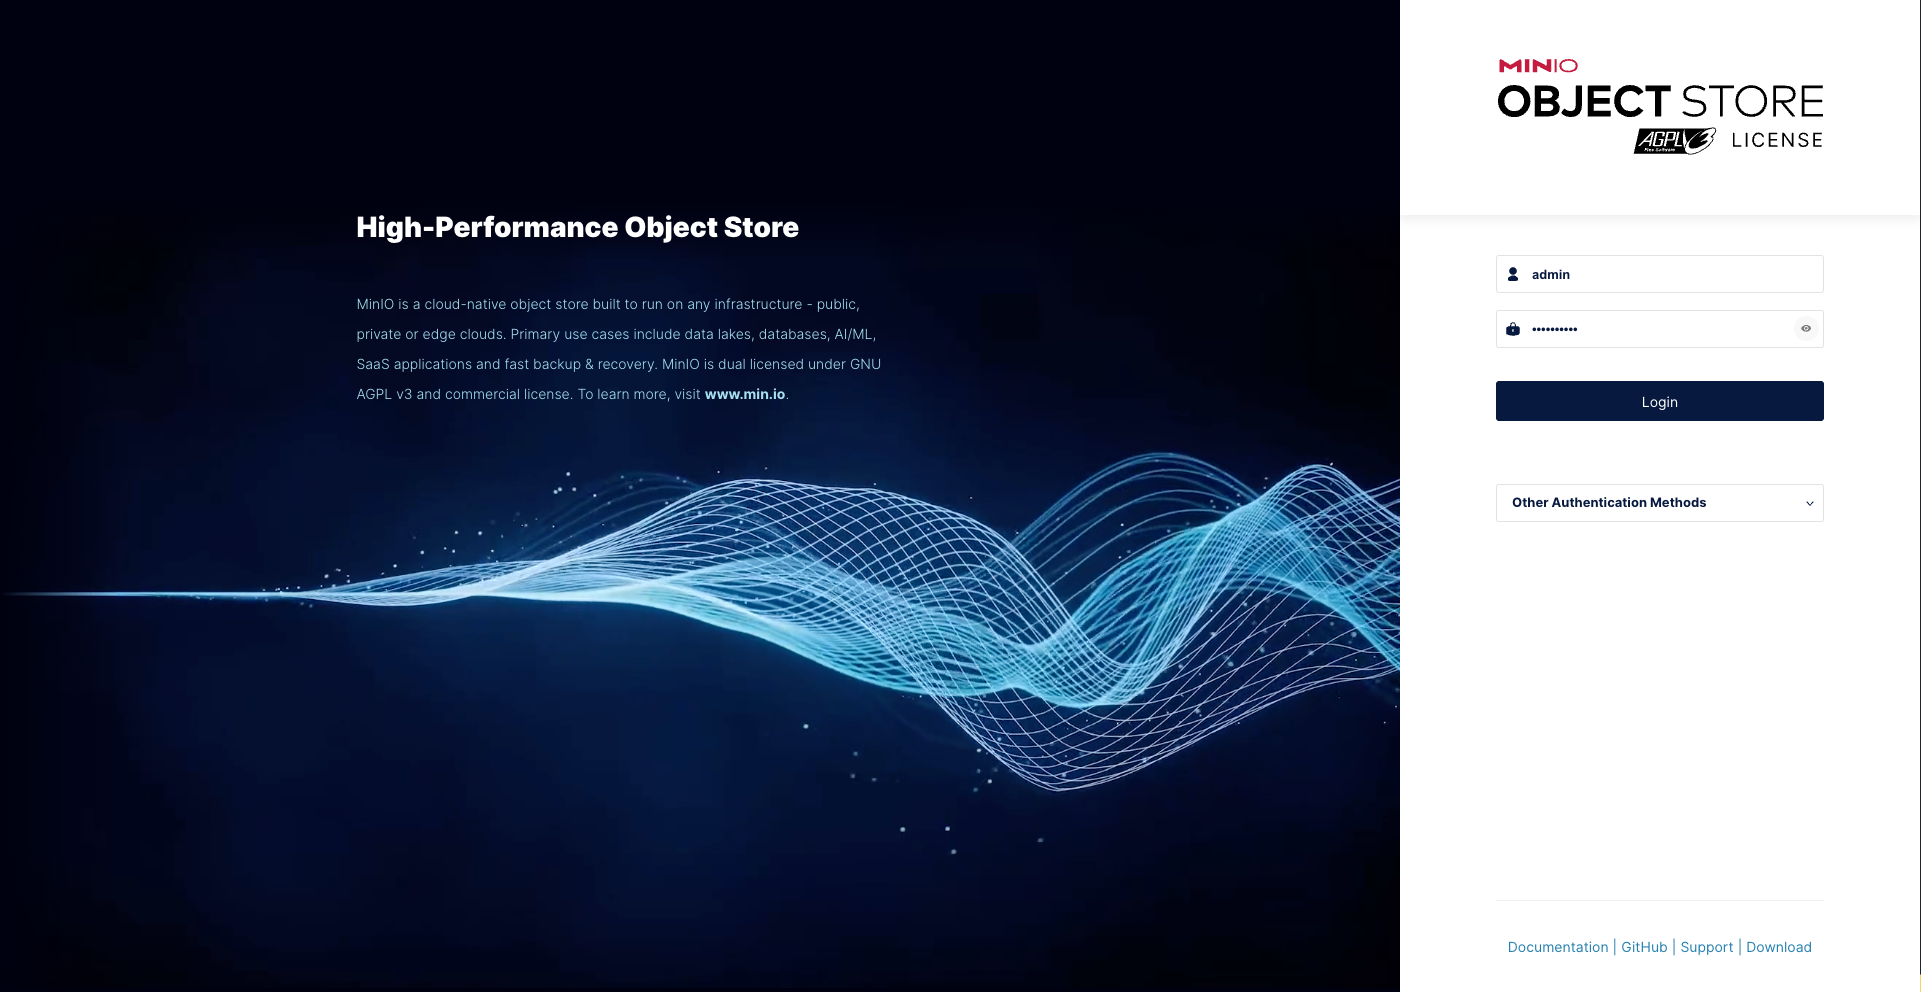
\includegraphics[width=1\linewidth]{graphics/minio-login.png}
    \caption[MinIO - Login Screen]{MinIO - Login Screen.}
    \label{fig:MinIO-Login}
\end{figure}

Nach erfolgreicher Einrichtung zeigt die MinIO-Oberfläche den konfigurierten Bucket \lstinline|lakehouse-storage|, wie in Abbildung \ref{fig:MinIO-Bucket} dargestellt. Dieser Bucket dient als zentraler Speicherort für Daten im Delta- und Parquet-Format, die im Rahmen der Lakehouse-Architektur verarbeitet und analysiert werden.

\begin{figure}[H]
    \centering
    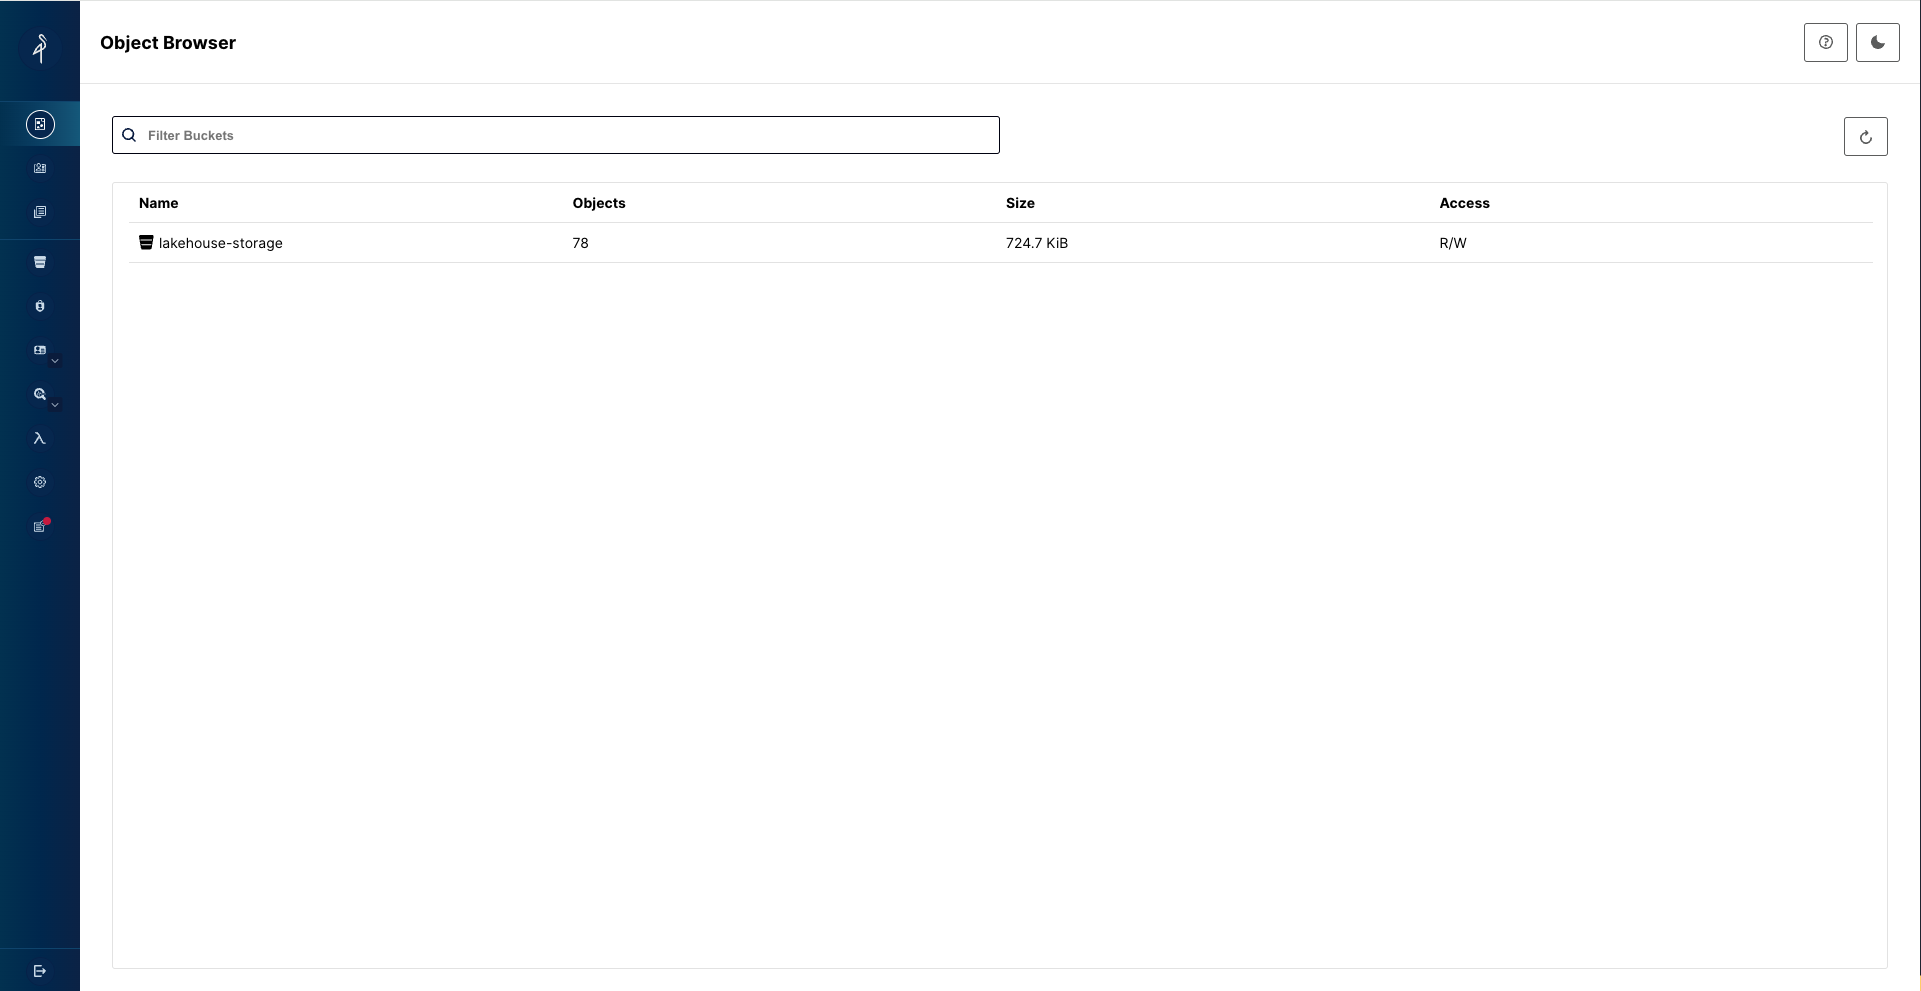
\includegraphics[width=1\linewidth]{graphics/minio.png}
    \caption[MinIO mit erstelltem lakehouse-storage Bucket]{MinIO mit erstelltem \lstinline|lakehouse-storage| Bucket.}
    \label{fig:MinIO-Bucket}
\end{figure}

Anschließend wird ein Spark-Cluster gestartet, bestehend aus einem \lstinline|spark-master|-Container, einem \lstinline|spark-worker|-Container und einem \lstinline|spark-submit|-Container. Dieser Cluster übernimmt die Verarbeitung der Ursprungsdaten aus der Datei \lstinline|ds_salaries.csv|. Dabei werden die Daten in Delta-Tabellen zerlegt und in den MinIO-Speicher hochgeladen, um eine effiziente Speicherung und Weiterverarbeitung zu gewährleisten. Dies markiert den ersten Schritt innerhalb einer Medallion-Architektur, in dem die "Raw" Daten verarbeitet, in Delta-Tabellen überführt und im gemeinsamen Speicher organisiert werden. Gleichzeitig erfolgen erste Transformationen, die die Grundlage für nachfolgende Verarbeitungsschritte bilden. Zudem wird dadurch eine Simulationsumgebung geschaffen, die demonstriert, wie Daten aus verschiedenen Systemen in ein Speicher geladen werden können.

Abbildung \ref{fig:Spark-Cluster} zeigt die Oberfläche des Apache Spark Clusters, die den Status und die laufenden Jobs visualisiert.

\begin{figure}[H]
    \centering
    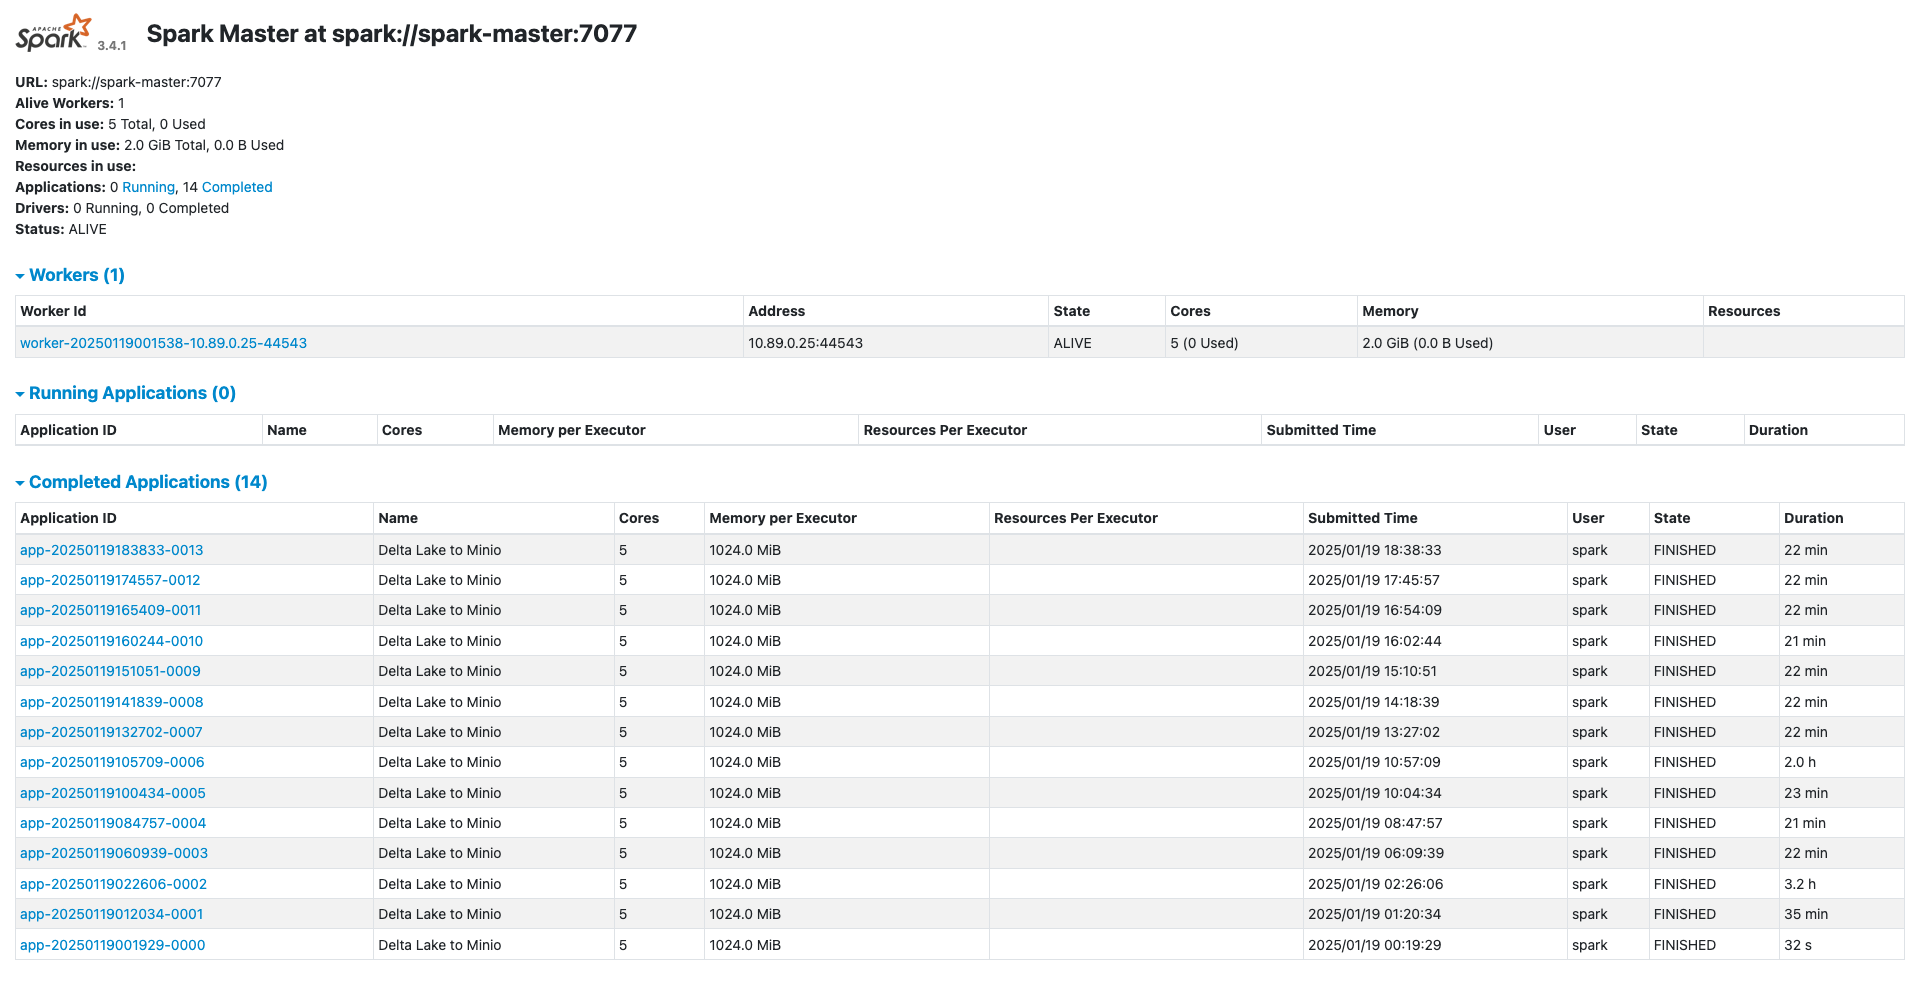
\includegraphics[width=1\linewidth]{graphics/spark.png}
    \caption[Oberfläche des Apache Spark Clusters]{Oberfläche des Apache Spark Clusters.}
    \label{fig:Spark-Cluster}
\end{figure}

Zur Anreicherung des Datensatzes mit zusätzlichen Informationen wird der \lstinline|scraper|-Container eingesetzt. Dieser sammelt Gehaltsdaten von der Webseite Glassdoor, verarbeitet sie mithilfe der Python-Bibliothek \lstinline|pandas| und der Bibliothek \lstinline|Selenium| und fügt sie dem bestehenden Datensatz hinzu (siehe Abbildung \ref{fig:Scraper}). Um eine regelmäßige Aktualisierung der Daten zu gewährleisten, sind sowohl der \lstinline|scraper|-Container als auch der \lstinline|spark-submit|-Container so konfiguriert, dass sie alle 20 Minuten automatisch ausgeführt werden. Dadurch bleibt der MinIO-Speicher stets auf dem neuesten Stand.

\begin{figure}[H]
    \centering
    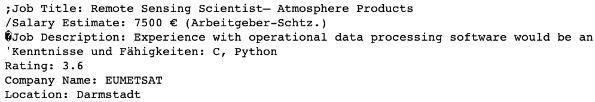
\includegraphics[width=0.8\linewidth]{graphics/scraper.png}
    \caption[Ein Ausschnitt einer gescrapten Jobstelle von Glassdoor]{Ein Ausschnitt einer gescrapten Jobstelle von Glassdoor.}
    \label{fig:Scraper}
\end{figure}

Die verarbeiteten Daten werden im MinIO-Speicher in Form von Delta Lake Tabellen gespeichert, wie in Abbildung \ref{fig:Delta-Tables} dargestellt. Diese Tabellen sind in verschiedene logische Partitionen unterteilt, was eine flexible Abfrage und Analyse ermöglicht.

\begin{figure}[H]
    \centering
    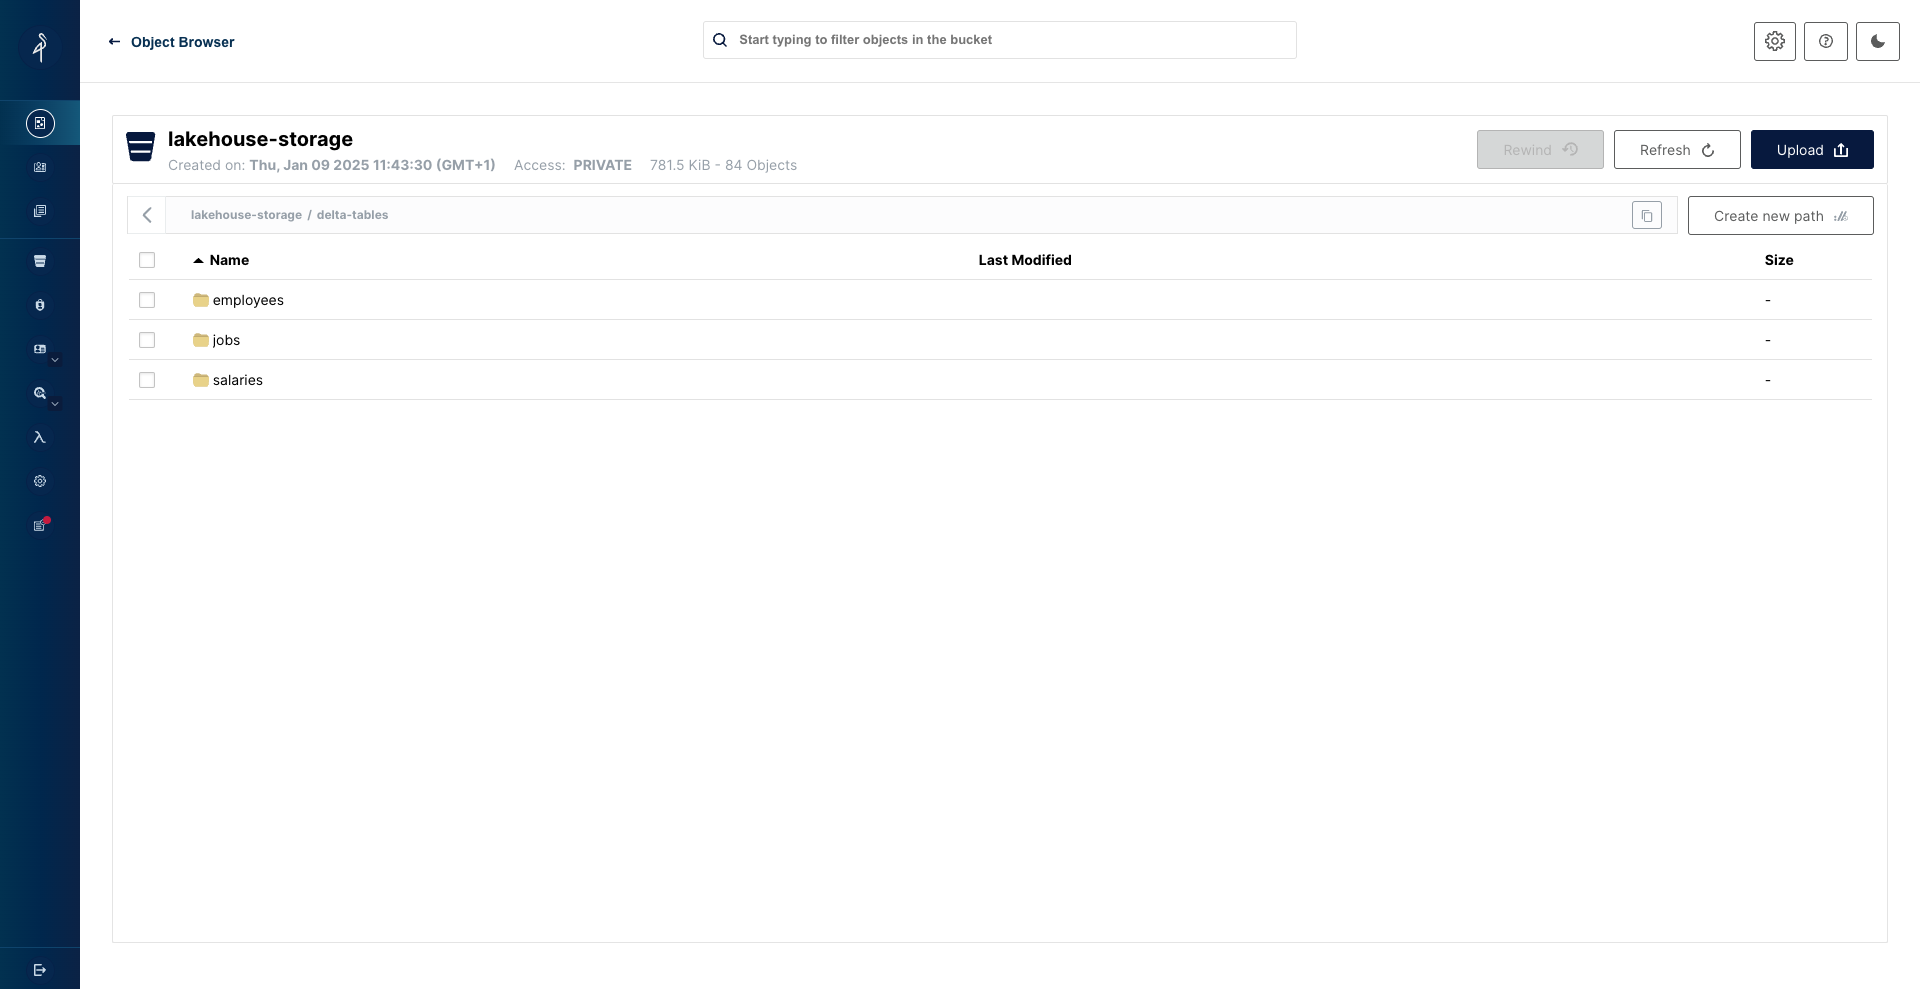
\includegraphics[width=1\linewidth]{graphics/delta-folder.png}
    \caption[Zerlegte CSV-Datei in Delta Lake Tabellen]{Zerlegte CSV-Datei in Delta Lake Tabellen.}
    \label{fig:Delta-Tables}
\end{figure}

Eine detaillierte Ansicht der gespeicherten Daten zeigt die Employee-Tabelle, die aus mehreren Parquet-Dateien besteht. Diese Dateien ermöglichen eine effiziente Speicherung und Bereitstellung großer Datenmengen, wie in Abbildung \ref{fig:Delta-Employee-Table} illustriert.

\begin{figure}[H]
    \centering
    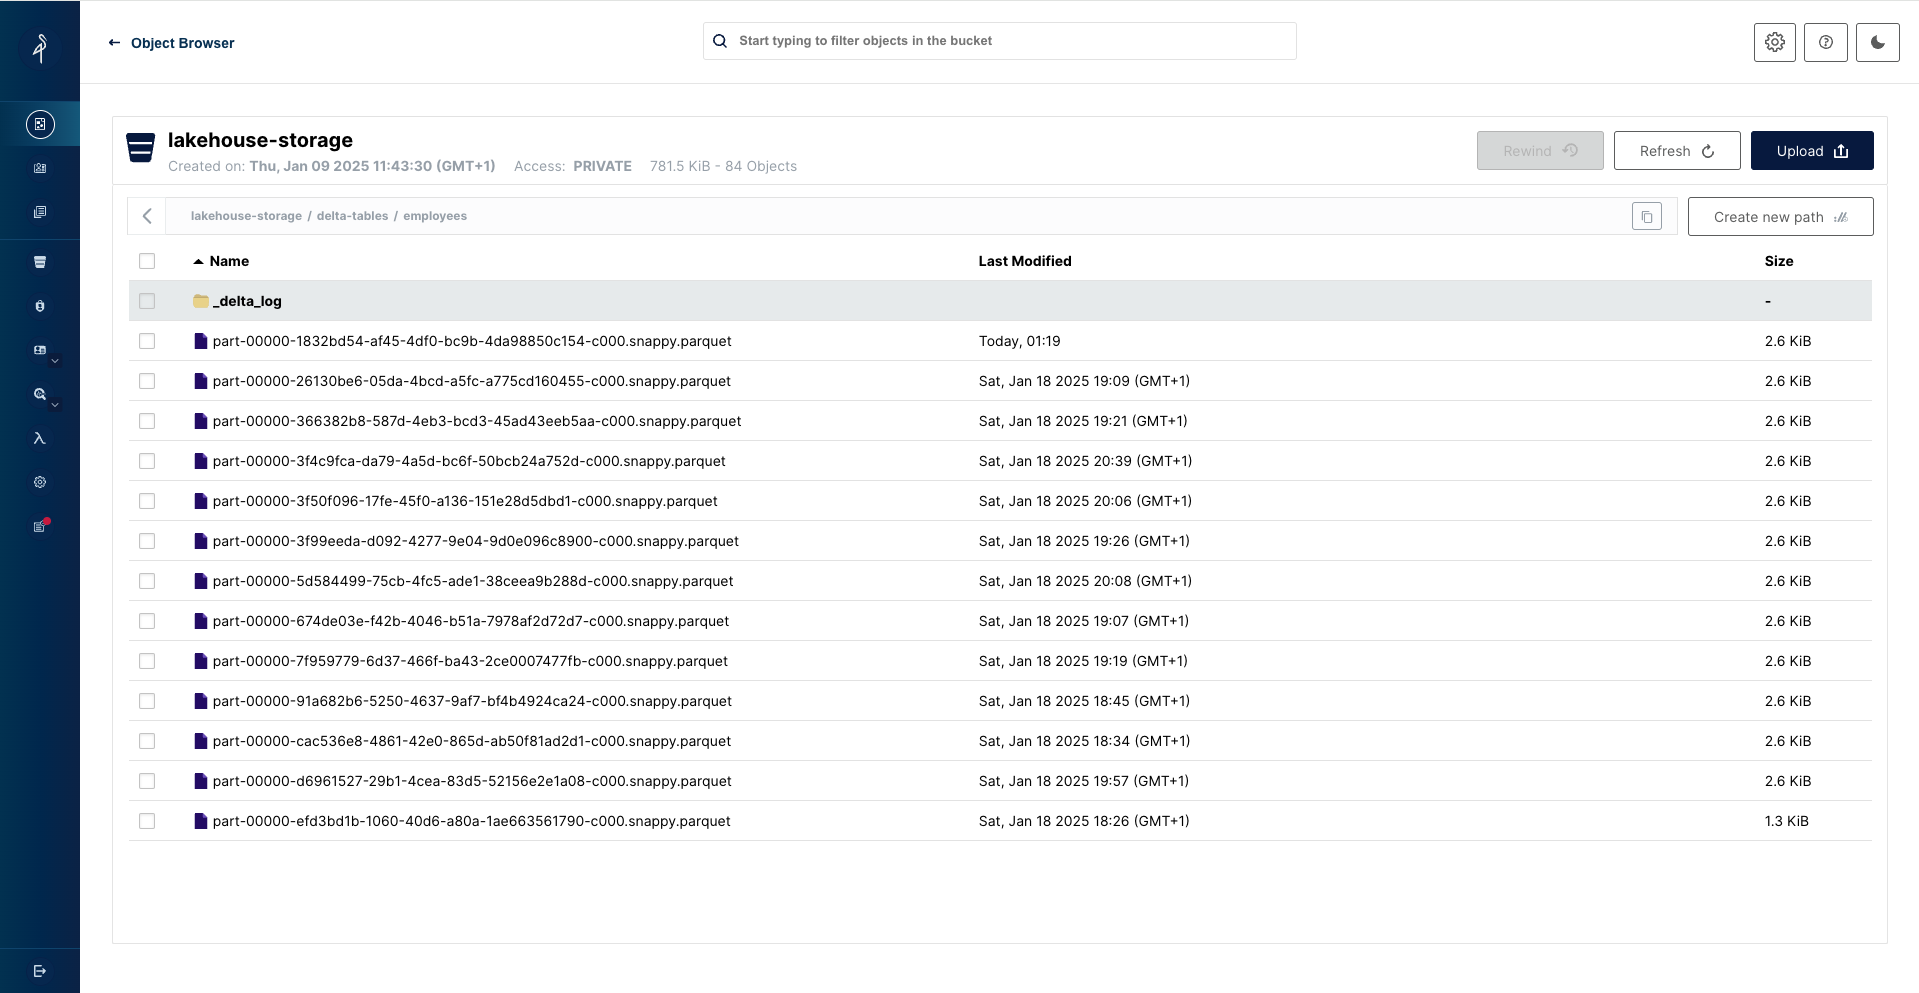
\includegraphics[width=1\linewidth]{graphics/delta-folder-employees.png}
    \caption[Delta Lake Employee Tabelle mit Parquet-Dateien]{Delta Lake Employee Tabelle mit Parquet-Dateien.}
    \label{fig:Delta-Employee-Table}
\end{figure}

Die drei Delta-Tabellen werden von DuckDB eingelesen und anschließend mit Ibis zusammengeführt, verarbeitet und analysiert. Die dabei erstellten Analysen bieten wertvolle Einblicke für geschäftliche Anwendungen und repräsentieren das Gold-Layer der Medallion-Architektur. 

\begin{figure}[H]
    \centering
    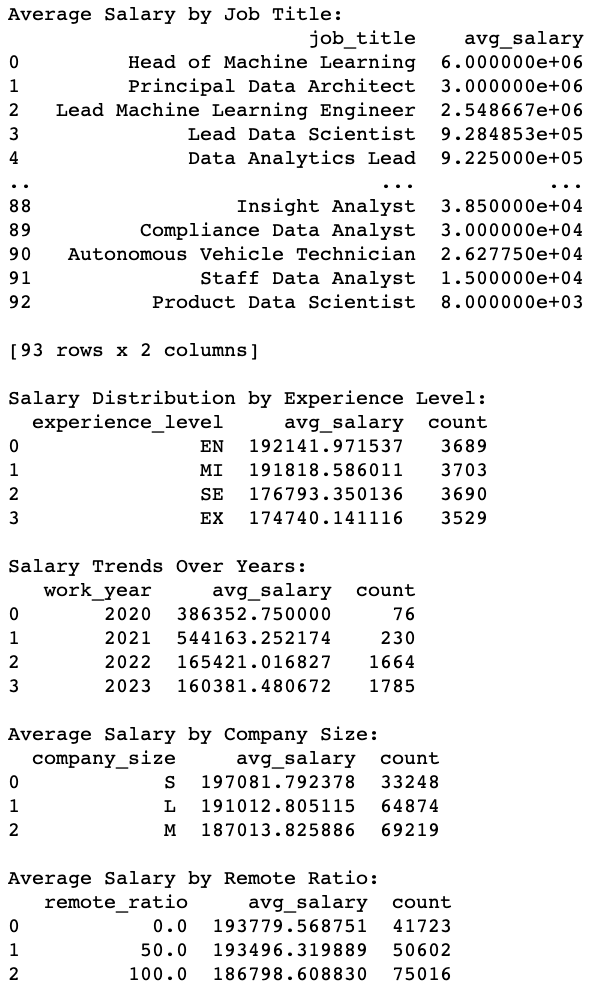
\includegraphics[width=0.5\linewidth]{graphics/analysen.png}
    \caption[Analysen mittels DuckDB und Ibis zur Visualisierung in Apache Superset]{Analysen mittels DuckDB und Ibis zur Visualisierung in Apache Superset.}
    \label{fig:Delta-Employee-Table}
\end{figure}

Die Visualisierung der Analyseergebnisse wird in Apache Superset realisiert, wo Dashboards und Diagramme erstellt werden, um detaillierte Einblicke in Gehaltsstrukturen und Arbeitsbedingungen zu bieten. Dieser Schritt bildet den Abschluss der Medallion-Architektur und demonstriert die vollständige Umsetzung einer Lakehouse-Architektur.

Aus den erstellten Charts und Dashboards lassen sich wertvolle Erkenntnisse ableiten, die eine fundierte Grundlage für strategische Entscheidungen bieten. 
Das erste Diagramm (Abbildung \ref{fig:chart1}) zeigt die durchschnittlichen Gehälter nach Jobtiteln und verdeutlicht, welche Rollen innerhalb des Bereichs Data Science am höchsten vergütet werden. Diese Analyse kann dazu genutzt werden, strategische Personalentscheidungen zu treffen oder Gehaltspakete wettbewerbsfähig zu gestalten.

\begin{figure}[H]
    \centering
    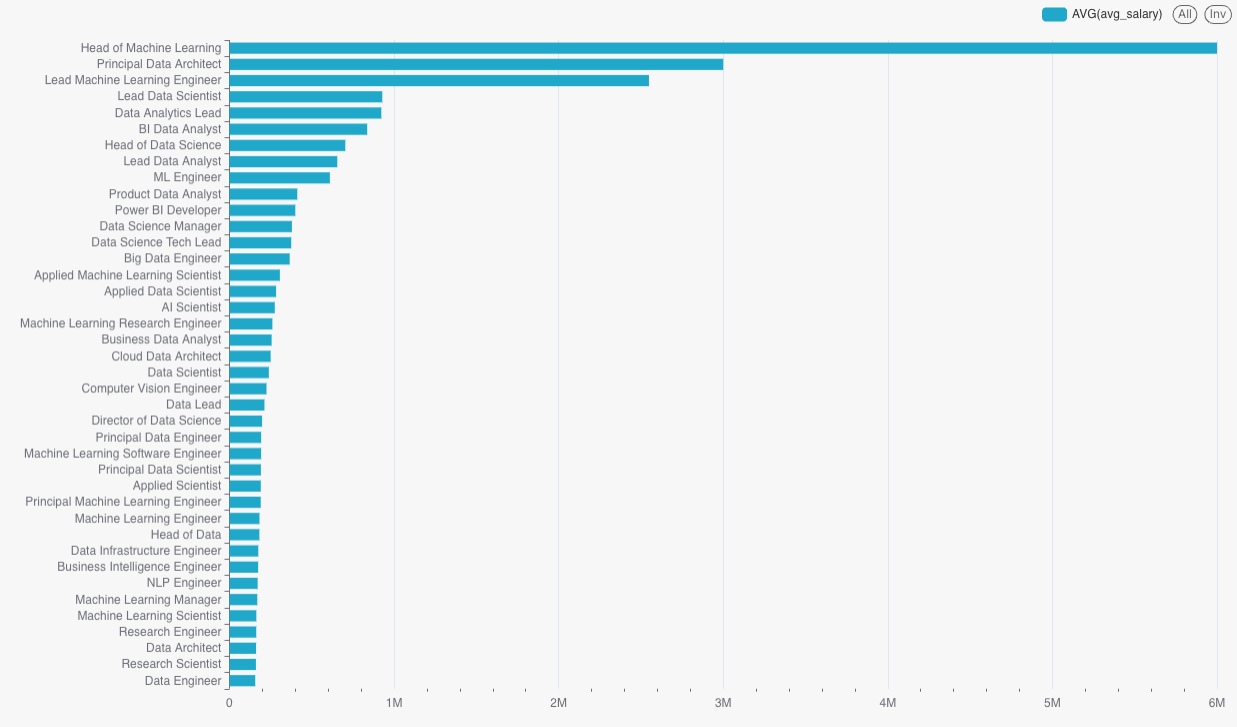
\includegraphics[width=1\linewidth]{graphics/salary-by-job.jpg}
    \caption[Durchschnittsgehälter nach Jobpositionen]{Durchschnittsgehälter nach Jobpositionen.}
    \label{fig:chart1}
\end{figure}

Das zweite Diagramm (Abbildung \ref{fig:Salary-over-years}) zeigt die Gehaltsentwicklung über die Jahre. Es wird ersichtlich, wie sich die durchschnittlichen Gehälter im Zeitverlauf verändert haben. Besonders auffällig ist der Höhepunkt im Jahr 2021, gefolgt von einem deutlichen Rückgang in den darauffolgenden Jahren, dies könnte jedoch auch auf fehlende Daten in diesem Jahr zurückzuführen sein. 

\begin{figure}[H]
    \centering
    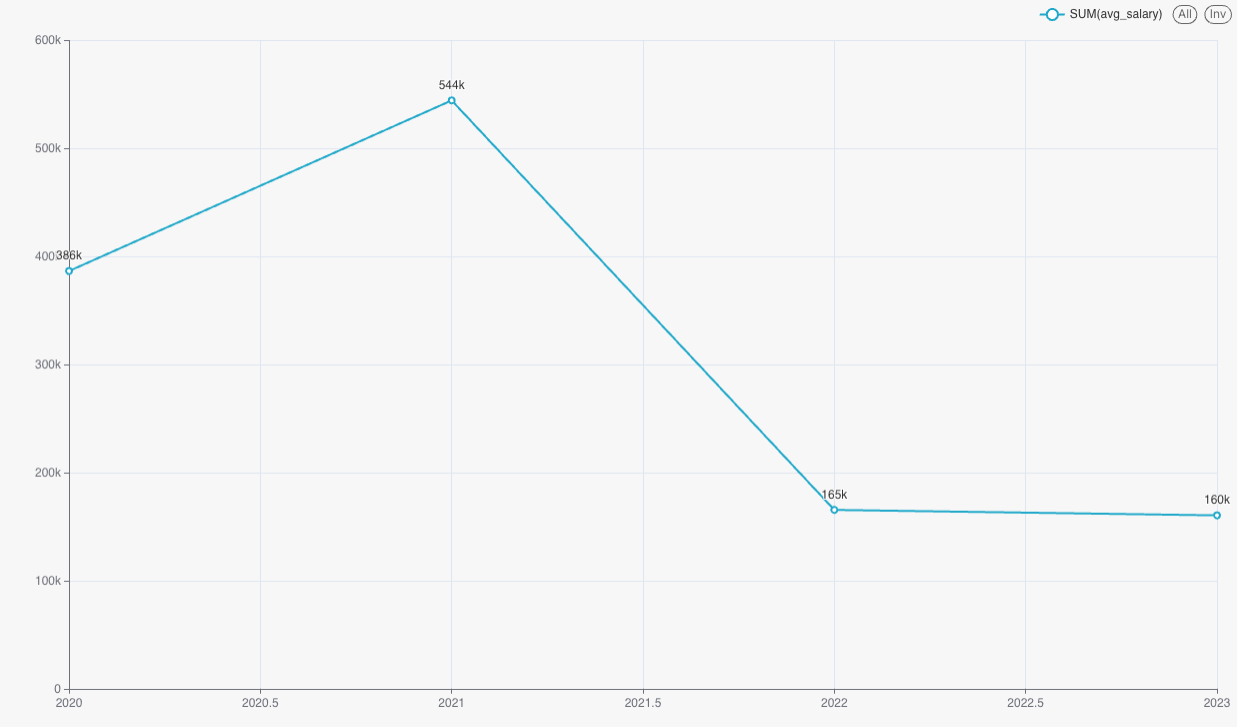
\includegraphics[width=0.8\linewidth]{graphics/salary-trend-year.jpg}
    \caption[Durchschnittliche Gehaltsentwicklung bei Data Science Jobs über die Jahre]{Durchschnittliche Gehaltsentwicklung bei Data Science Jobs über die Jahre.}
    \label{fig:Salary-over-years}
  \end{figure}

\newpage  

Im Anhang sind drei weitere Diagramme aus den Analysen mit DuckDB, Ibis und Apache Superset dargestellt (siehe Anhang \ref{anhang:zusaetlichediagramme}). Diese Visualisierungen verdeutlichen die Vielseitigkeit und den Mehrwert der in der Lakehouse-Architektur implementierten Datenanalyse.

Abschließend bleibt anzumerken, dass die Konfiguration von Apache Superset den einzigen manuellen Schritt innerhalb der Umsetzung darstellt. Dabei müssen Datenquellen und Dashboards eingerichtet werden, um benutzerspezifische Visualisierungen zu ermöglichen. Während dieses Prozesses trat ein nicht behebbarer Fehler auf. Das Hinzufügen von Charts zu einem Dashboard führte wiederholt zu einem Core Dump, siehe Anhang \ref{anhang:apachesuperset}. Weder die Log-Analyse noch Tests auf unterschiedlichen Endgeräten konnten das Problem lösen, was auf einen möglichen Fehler in Apache Superset hinweist. Dennoch konnte die Funktionalität der Lakehouse-Architektur erfolgreich demonstriert werden, da die Visualisierung der Daten weiterhin über die Erstellung von Charts möglich war.

